\chapter{Adoption, policy and outlook}
\label{ch:outlook}

\begin{objectives}\small
\begin{itemize}[nosep,leftmargin=*]
  \item survey where this practice is already adopted, and the policy that backs it;
  \item situate Software Heritage in the resilience, sovereignty, and transparent-AI agendas;
  \item identify what to do as a researcher, a reviewer, or an institution.
\end{itemize}
\end{objectives}

We have built the argument and shown the practice. It remains to look outward: to see that this is
already happening, that policy now stands behind it, and that the same infrastructure serves a
mission far larger than open science. And then to ask what you can do, starting --- one last time
--- with your next paper.

\takeaway{Open science is one payoff of software preservation; resilience, transparency, and
sovereignty are others.}

\section{It is already happening}

None of this is hypothetical. Journals and platforms across disciplines have wired Software Heritage
into how they work: the HAL national repository offers a curated software-deposit workflow; IPOL
publishes image-processing papers with runnable code and a SWHID; \emph{eLife} archives the code
behind every article automatically; \emph{swMATH} references mathematical software in the archive;
and Episciences journals such as JTCAM ask authors to cite their software with
\texttt{biblatex-software} (itself shipped in the ACM article class since
2022)~\autocite{SwhCACM2018}. The connections keep multiplying: Episciences now links each published
article to its code through a \textsc{swhid}~\autocite{episciences2025swh}; \emph{Zenodo} forwards
its software deposits to the archive (Chapter~\ref{ch:ardc}); and code-publishing venues such as
Dagstuhl's \emph{DROPS} interconnect the same way.\footnote{\url{https://drops.dagstuhl.de/}.} Papers
themselves now carry not one identifier but many, pinpointing their code passages with qualified
\textsc{swhid}s throughout the text~\autocite{spinellis2026hotspots}.

And the stakes are real, not niche. When the French ministry surveyed its research-software
producers, the picture that emerged was of long-lived, widely-used, high-impact work: half of the
software reported was more than nine years old, a third had over a hundred users, and nearly
two-thirds had impact beyond academia --- overwhelmingly released as free and open
source.\footnote{French Ministry of Higher Education and Research, research-software survey, 2023.}
This is not a fringe of scientific practice; it is a load-bearing part of it, and it has been going
uncared-for.

\section{The policy that backs it}

The direction of travel, at every level, is now unambiguous. The \textbf{UNESCO Recommendation on
Open Science} (2021) calls for source code to be released openly, and for open-science
infrastructures to be \enquote{organized and financed upon an essentially not-for-profit and
long-term vision}~\autocite{UNESCO2021OpenScience}. The European \textbf{EOSC SIRS report} (2020) is
more specific still: \emph{archive in Software Heritage, use the SWHID}, and treat open source as the
default for research software, with deviations to be justified~\autocite{SIRSReport2020}. The
\textbf{Paris Call on Software Source Code} (2019) had already urged the world to \enquote{recognise
software source code as a fundamental enabler in all aspects of human endeavour} and to build shared
infrastructures to preserve it~\autocite{ParisCall2019}. And at the national level the message is the
same: France's second \textbf{National Plan for Open Science} names Software Heritage and the
\textsc{swhid} explicitly, the country's research-infrastructure roadmap now lists the archive, and a
standing College for research software carries the agenda forward~\autocite{PNSO2_2021,osec_2022}.
Strip away the acronyms and a single instruction remains: archive in Software Heritage, and identify
with a \textsc{swhid}.

\begin{figure}[htbp]
  \centering
  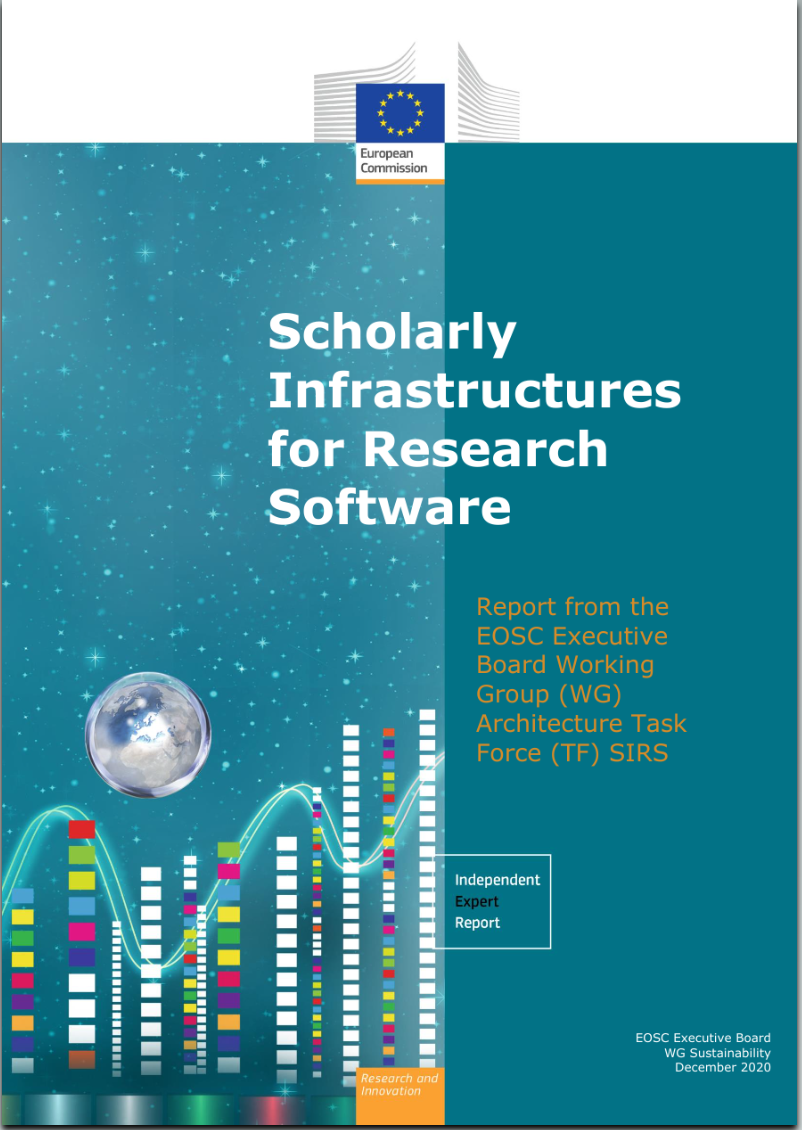
\includegraphics[height=5.3cm]{figures/EOSC-SIRS-report.png}\hspace{7mm}
  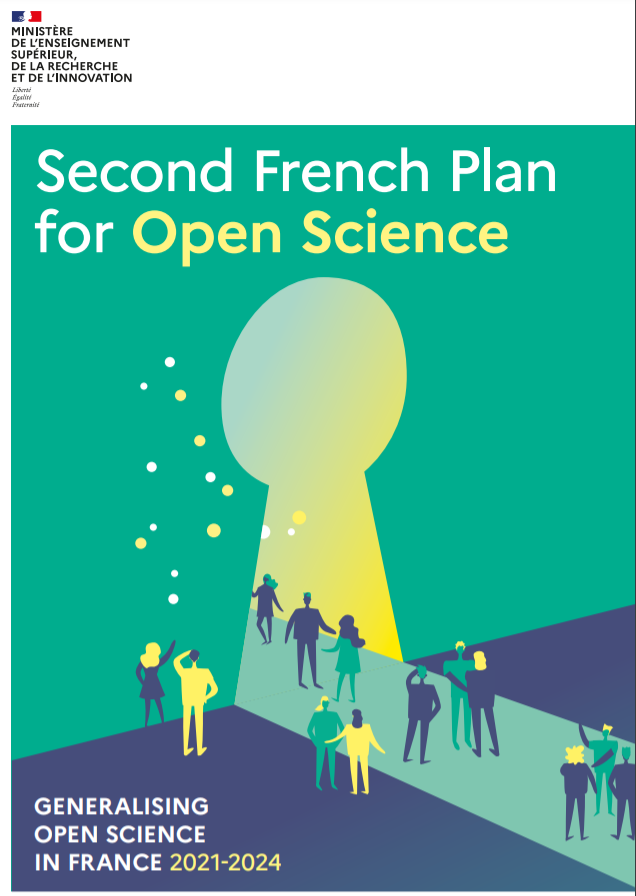
\includegraphics[height=5.3cm]{figures/PNSO2-en-cover.png}
  \caption[Policy documents]{Two of the documents that now point research software at Software
  Heritage: the EOSC \emph{Scholarly Infrastructures for Research Software} report (left,
  2020)~\autocite{SIRSReport2020} and France's second National Plan for Open Science (right,
  2021--2024)~\autocite{PNSO2_2021}.}
  \label{fig:policy}
\end{figure}

Funders have followed. France's national research agency, the ANR, asks in its own funding
guidelines that project software be released under a libre licence and its source archived in
Software Heritage, with the grant referenced (Figure~\ref{fig:anr}).

\begin{figure}[htbp]
  \centering
  \fbox{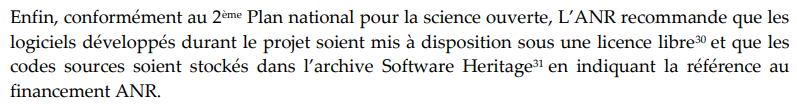
\includegraphics[width=.96\linewidth]{figures/anr-recommendations.png}}
  \caption[ANR funding guideline]{From the ANR's funding guidelines: project source code is to be
  stored in Software Heritage under a free licence, with the ANR grant referenced.}
  \label{fig:anr}
\end{figure}

\takeaway{The policy is unambiguous: archive in Software Heritage, identify with a \textsc{swhid}.}

\section{The wider mission: resilience, sovereignty, transparent AI}

Open science is only one of the things this archive makes possible, and stepping back reveals why it
matters beyond the library. The same uniform record of the world's source code is the foundation for
several urgent agendas at once. It underpins \emph{software supply-chain traceability}: an
intrinsic identifier is exactly what a software bill of materials (an \textsc{sbom}) needs, and what
regulators reaching for the EU Cyber Resilience Act will
require~\autocite{EU_CRA_2024,barais2025swhidcyber}. It underpins
\emph{transparent AI}: the very large code corpora that train today's models --- The Stack, on which
StarCoder is built --- are drawn from Software Heritage, and provenance for that data is becoming a
legal as well as an ethical demand~\autocite{StarCoder2_2024}. And it underpins \emph{resilience}:
because the archive holds the code with its history, a build system can fall back to it when the
upstream platform fails. Guix has done exactly this since 2019 --- when a package vanishes from its
registry, the build continues from Software Heritage~\autocite{dicosmo_tpdl_2022,SWHecosystems2023}.
The point is not academic. If GitHub or PyPI disappeared tomorrow, much of the digital world would
not merely slow down --- it would stop.

This reframes the whole enterprise. The goal is not to \emph{own} the infrastructure but to ensure
that nothing essential can vanish --- a shared, open, non-rival archive that benefits all while
leaving each free to build on it. That is digital sovereignty rightly understood: not autarky, but
\emph{resilience}.

\section{A fair question: what about Software Heritage itself?}

This note has argued that platforms fail and that we should plan for it --- so it must turn the same
lens on the archive it recommends. Software Heritage is a non-profit initiative launched in 2016,
hosted by Inria and run as an international, multi-stakeholder effort under an agreement with UNESCO;
it is funded by a range of institutional members and sponsors rather than by any single company or
state, with foundational support from bodies such as the Alfred P.\ Sloan and NLnet foundations. Its
answer to its own single-point-of-failure risk is a \emph{network of independent mirrors} --- full
copies of the archive held by partner institutions, so the corpus survives the loss of any one
operator. It is the same resilience-by-redundancy the archive offers your build chain, turned on
itself. For an editor or a funder weighing a ten-year commitment, that --- not a metaphor --- is the
due-diligence answer.

It is equally worth being clear about the \emph{limits}. A \textsc{swhid} secures the \emph{identity}
and \emph{availability} of source code; it does not make a build deterministic
(Chapter~\ref{ch:repro}), and it cannot open code that was never public. Adoption, though real and
growing, is still offered as one option among several at most venues rather than a default. The
claim of this note is not that the work is finished --- it is that the infrastructure, the standard,
and the practice are now ready to be made the default.

\section{Call to action}

Which brings us, finally, back to you. The tools are built, the policy is written, the adoption is
under way; the one thing still missing is the habit. So make it, at three scales.

\emph{As a researcher:} archive the code behind your next result in Software Heritage, reference it
with a \textsc{swhid} at the granularity your claim needs, describe it, and cite it. That is the
whole of \textsc{ardc}, and you can do it this week.

\emph{As a reviewer, an editor, or a member of an artifact-evaluation committee:} ask authors for
archival proof --- a \textsc{swhid} --- rather than a fragile URL. It is one small habit, but applied
every time, it changes the norms of a whole community.

\emph{As an institution or a funder:} write Software Heritage into your open-science policy, become a
member or run a mirror, and --- not least --- count high-quality software contributions in the
careers of the people who make them.

\begin{callout}{Ready to paste: a grant condition and a policy line}
\small \textbf{Grant condition} (it costs the grantee nothing --- archival is free):
\begin{quote}\itshape
Source code produced with this grant must be released under an open licence and archived in Software
Heritage, and the resulting \textsc{swhid} reported in the project's outputs. (Further documentation,
testing, and packaging are encouraged but not required.)
\end{quote}
\textbf{Open-science / sovereignty policy line:}
\begin{quote}\itshape
We adopt intrinsic, standard identifiers (\textsc{swhid}, ISO/IEC~18670) and a shared, non-profit
archive (Software Heritage) for research software, ensuring that publicly funded code remains
verifiable, citable, and recoverable independently of any commercial platform.
\end{quote}
A funder can audit compliance across a whole portfolio with one HAL-API call
(\S\,\ref{ch:ardc}'s \texttt{collCode\_s} query), no per-project chasing required.
\end{callout}

Software source code is a precious, unique form of knowledge, and for too long we have treated it as
an afterthought. We no longer have to. The argument is settled and the machinery is ready; what is
needed now is simply that we use it. Record your code, share it, and value
it~\autocite{NatureSD2026}. Start with your next paper.
